\chapter{Methodology}
\label{chap:methodology}

Research methodology serves as the systematic framework that guides how complex technical investigations are conducted, problems are analyzed, and solutions are developed and evaluated. For a project situated at the intersection of affective computing and large language models (LLMs), a robust methodology is critically important to navigate the inherent complexities of both human emotion and computational systems. It provides a structured pathway that ensures rigor in experimentation, credibility in results, and replicability for the academic community. This framework is essential for achieving both academic validation through novel knowledge contributions and practical implementation through the creation of a useful, well-engineered artifact. 

The goal of this research to design, build, and evaluate a novel hybrid retrieval system to enhance N-shot context learning for emotion classification necessitates a methodology that is both structured and adaptive. For this reason, \textbf{Design Science Research (DSR)} has been selected as the guiding framework. DSR is uniquely suited for this work as its core tenets are centered on the creation and evaluation of innovative artifacts to solve real-world problems, making it the ideal approach for a project that aims to produce a tangible computational solution \cite{hevner2004design,peffers2007dsr}.

\section{Design Science Research Method}
\label{sec:dsrm-overview}

\subsection{DSR Fundamentals}
Design Science Research (DSR) is a well-established research paradigm in the information systems and computer science disciplines that is fundamentally concerned with the creation of innovative artifacts to solve practical problems \cite{hevner2004design}. Unlike natural sciences, which seek to understand and explain reality, design science seeks to ``create things that serve human purposes'' \cite{simon1996sciences}. The DSR methodology provides a framework for conducting research that is both academically rigorous and practically relevant, making it exceptionally well-suited for applied technical projects. 

The research process is guided by several principles:

\begin{itemize}
    \item \textbf{Problem-Oriented Focus:} DSR begins with identifying and clearly articulating a relevant technical problem. Here, the problem is the performance instability and sub-optimal accuracy of standard N-shot learning for emotion classification, which is often limited by poorly chosen in-context examples \cite{zhao2021calibrate}.
    \item \textbf{Artifact-Centric Approach:} The primary output of DSR is a purposeful artifact, which may be a construct, model, method, or instantiation \cite{hevner2004design}. In this research, the artifact is the \textbf{hybrid retrieval system}, a working software prototype that combines the lexical precision of BM25 with the semantic nuance of cosine similarity to select high-quality examples for N-shot prompting.
    \item \textbf{Rigorous Evaluation:} The utility and efficacy of the designed artifact must be rigorously demonstrated. This project evaluates the hybrid retrieval system using macro F1-score comparisons of GPT-4 classifications on the GoEmotions dataset \cite{demszky2020goemotions}.
    \item \textbf{Iterative Refinement:} DSR is an iterative process of design, build, and evaluation cycles \cite{peffers2007dsr}. Feedback from evaluations informs subsequent refinements of the artifact.
    \item \textbf{Knowledge Contribution:} A DSR project must provide contributions to the knowledge base, either through the artifact itself or through design principles derived from its creation and evaluation \cite{gregor2013positioning}. This research contributes both a system and new insights into hybrid retrieval for affective computing tasks.
\end{itemize}

\subsection{DSR Iterative Process}
This project adopts the five-phase cycle from \cite{peffers2007dsr}, as illustrated in Figure~\ref{fig:dsrm_process}.

\begin{figure}[H]
    \centering
    \includegraphics[width=0.8\textwidth]{Images/DSRcycle.PNG}
    \caption{Adapted DSRM process for hybrid retrieval system development.}
    \label{fig:dsrm_process}
\end{figure}


\newpage

\paragraph{Phase 1: Problem Investigation.}
The first step involved clarifying the research problem and its practical relevance. Through a review of recent work on large language models, the challenge of inconsistent and unstable results in few-shot emotion classification became apparent. This established a clear gap where existing approaches failed to provide reliable performance, thereby justifying the need for a novel solution.

\paragraph{Phase 2: Solution Design.}
In response to the identified problem, a potential solution concept was outlined. The guiding principle was that any effective design should enhance both accuracy and stability of emotion classification. At this stage, success criteria were defined in terms of measurable improvements in performance outcomes while ensuring the system remained adaptable to varied contexts.

\paragraph{Phase 3: Design Validation.}
The next step focused on evaluating whether the proposed solution could realistically address the problem. This required aligning the system’s design goals with theoretical insights from the literature and ensuring that the architecture was robust, scalable, and implementable. By confirming its feasibility, the foundation was laid for subsequent development.

\paragraph{Phase 4: Solution Implementation.}
Once validated, the solution was implemented in a structured manner. This involved transforming the conceptual design into a functional system that could be demonstrated in practice. The system was deployed in a controlled environment where its ability to handle real-world scenarios could be observed and refined as needed.

\paragraph{Phase 5: Solution Evaluation.}
Finally, the implemented solution was systematically evaluated against established benchmarks and baseline approaches. The focus here was on determining whether the solution truly delivered improvements in terms of effectiveness, reliability, and stability. Multiple evaluations were carried out to ensure that the findings were credible and provided a sound basis for drawing meaningful conclusions.
\subsection{Application to Affective Computing and NLP}
In affective computing and NLP, artifacts such as datasets and algorithms are themselves major contributions \cite{hirschberg2015advances}. DSR provides the necessary structure for building artifacts that are both theoretically grounded and practically evaluated. The adaptation here emphasizes quantitative benchmarking on GoEmotions rather than user studies, aligning with NLP research norms.

\section{Research Design and Implementation Approach}
\label{sec:research-design}

\subsection{Problem Investigation}
The systematic literature review (2019–2025) revealed under-exploration of hybrid retrieval in Retrieval-Augmented Generation (RAG) for N-shot learning \cite{lewis2020retrieval,karpukhin2020dense}. The project success criterion is a statistically significant macro F1 improvement over semantic-only retrieval.

\subsection{Solution Design Framework}
The solution is designed around modularity and reproducibility:

\begin{itemize}
    \item \textbf{Modules:} Data Processing (GoEmotions), Baseline Retrieval (semantic), Hybrid Retrieval (BM25 + embeddings), N-shot Prompting, LLM Interaction (Azure GPT-4), and Evaluation.
    \item \textbf{Principle:} The baseline and hybrid systems share all components except retrieval, isolating the impact of the artifact.
\end{itemize}

\subsection{Evaluation Framework}
Evaluation uses a quantitative, comparative setup:

\begin{itemize}
    \item \textbf{Metrics:} Macro F1 (primary), precision, recall, accuracy (secondary).
    \item \textbf{Design:} Comparison across three levels of granularity: 27 fine-grained labels, 15 clusters, and 3 sentiment groups. The optimal number of shots is guided by the stopping rule in \cite{zhu2020stopping}.
    \item \textbf{Baselines:} Random selection provides a lower bound; semantic-only serves as the comparative baseline.
\end{itemize}
\begin{figure}[H]
\centering
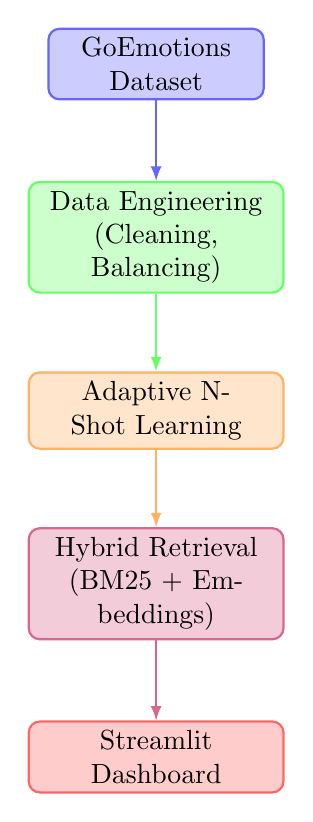
\begin{tikzpicture}[node distance=2.2cm,>=latex]
\node (input) [draw, rounded corners, text width=2.5cm, align=center, fill=blue!20, draw=blue!60, thick] {GoEmotions Dataset};
\node (clean) [draw, rounded corners, below of=input, text width=3cm, align=center, fill=green!20, draw=green!60, thick] {Data Engineering \\ (Cleaning, Balancing)};
\node (context) [draw, rounded corners, below of=clean, text width=3cm, align=center, fill=orange!20, draw=orange!60, thick] {Adaptive N-Shot Learning};
\node (retrieval) [draw, rounded corners, below of=context, text width=3cm, align=center, fill=purple!20, draw=purple!60, thick] {Hybrid Retrieval \\ (BM25 + Embeddings)};
\node (ui) [draw, rounded corners, below of=retrieval, text width=3cm, align=center, fill=red!20, draw=red!60, thick] {Streamlit Dashboard};

\draw[->, thick, blue!60] (input) -- (clean);
\draw[->, thick, green!60] (clean) -- (context);
\draw[->, thick, orange!60] (context) -- (retrieval);
\draw[->, thick, purple!60] (retrieval) -- (ui);
\end{tikzpicture}
\caption{Overall methodological pipeline connecting all components.}
\end{figure}
\section{Tools and Technologies}
\label{sec:tools-tech}

\begin{table}[H]
\centering
\caption{AI and Machine Learning Technologies}
\label{tab:ai_ml_tools}
\begin{tabular}{@{}p{4cm} p{5.5cm} p{5.5cm}@{}}
\toprule
\textbf{Technology} & \textbf{Purpose and Implementation} & \textbf{Justification} \\
\midrule
Python 3.9+ & Programming language for all components. & Standard for AI/ML research. \\
\addlinespace[0.3em]
GPT-4 DeepSeek-R1 Qwen3 (Azure) & N-shot emotion classification. & State-of-the-art LLMs with stable access \cite{openai2023gpt4}. \\
\addlinespace[0.3em]
Hugging Face Transformers & Access to all-MiniLM-L6-v2 model. & Standardized, high-performance embeddings. \\
\addlinespace[0.3em]
PyTorch & Backend for embedding model. & Flexible deep learning framework. \\
\addlinespace[0.3em]
Rank-BM25 & Lexical retrieval. & Efficient BM25 implementation. \\
\addlinespace[0.3em]
Pandas/NumPy & Data manipulation and preprocessing. & Core for data analysis in Python. \\
\addlinespace[0.3em]
Scikit-learn & Evaluation metrics. & Validated ML metrics library. \\
\addlinespace[0.3em]
Matplotlib/Seaborn & Visualization. & Publication-ready analysis. \\
\addlinespace[0.3em]
Streamlit & Web application framework for interactive demo. & Rapid prototyping and user-friendly interface \cite{streamlit2019}. \\
\bottomrule
\end{tabular}
\end{table}

\begin{table}[H]
\centering
\caption{Development and Quality Assurance Tools}
\label{tab:dev_tools}
\begin{tabular}{@{}p{4cm} p{5.5cm} p{5.5cm}@{}}
\toprule
\textbf{Technology} & \textbf{Purpose} & \textbf{Justification} \\
\midrule
Git \& GitHub & Version control. & Transparency and reproducibility. \\
JupyterLab & Experiment prototyping. & Supports iterative workflows. \\
Pytest & Unit testing retrieval modules. & Ensures correctness and reliability. \\
Python venv & Dependency management. & Guarantees reproducibility. \\
\bottomrule
\end{tabular}
\end{table}

\section{Methodological Rigor and Validation}
\label{sec:quality}
\subsection{Quality Assurance}
Rigor is ensured through multiple systematic approaches:
\begin{itemize}
    \item Git-based versioning for code management and reproducibility
    \item Pytest unit tests for component validation
    \item Detailed documentation for transparency and replication
    \item Automated scripts ensuring full experimental reproducibility
\end{itemize}

\subsection{Ethical Considerations}
The research adheres to established ethical principles:
\begin{itemize}
    \item The GoEmotions dataset consists of anonymized Reddit comments \cite{demszky2020goemotions}
    \item No personal data was collected during the study
    \item Ethical risks, particularly the misuse of emotion recognition, are acknowledged in the conclusion
    \item Transparency and open access to code form the core ethical commitments
    \item Full disclosure of potential limitations and biases in the system
\end{itemize}
\section{Conclusion}
\label{sec:summary}
This chapter presented the methodological framework for this research. Design Science Research was adopted due to its alignment with artifact-driven problem solving. The five-phase cycle was applied to design, implement, and evaluate a hybrid retrieval system for emotion classification. A rigorous research design ensured systematic investigation, while the tools and technologies supported reproducibility and robustness. Finally, ethical and quality assurance measures were embedded throughout the process, ensuring the research outcomes are both scientifically valid and socially responsible.
